\subsection{Comparison of Prediction Methods}

EG01-EG23, EG01-EG24, EG01-EG29, and EG01-EG30 transition scenarios
are set up in \Cyclus using \deploy. 
We ran each transition scenario with different prediction 
methods to determine the prediction method that best minimizes 
power undersupply for that scenario. 
We defined the EG01-EG23 and EG01-EG29 transition scenario simulations to have a constant 
power demand, while EG01-EG24 and EG01-EG30 have a linearly increasing power demand. 
Similar to the simple transition scenario, these transition scenario 
simulations begin with an initial fleet of \glspl{LWR} 
that start progressively decommissioning at the 80-year mark, 
after which \deploy deploys \glspl{SFR} and \gls{MOX} \glspl{LWR} to meet 
the power demand. 
Figure \ref{fig:eg2329}
shows the setup of facilities and mass flows for 
EG01-EG23 and EG01-EG29 in \Cyclus. 
In EG01-EG23 and EG01-EG29, recycled plutonium from LWR spent fuel 
produces  \gls{SFR} fuel. 
EG01-EG24 and EG01-EG30 are similar to EG01-EG23 and EG01-EG29, respectively, 
with the exception that all transuranic elements are recycled.

\begin{figure}[H]
	\centering
	\begin{subfigure}[t]{\textwidth}
		\centering
		\resizebox{0.6\textwidth}{!}{%
		\begin{tikzpicture}[node distance=2.5cm]
		\tikzstyle{every node}=[font=\normalsize]
		\node (source)[ollblock]{\texttt{Source}};
		\node (enrich)[ollblock, below of=source]{\texttt{Enrichment}};
		\node (lwr)[ollblock, below of=enrich]{\texttt{LWR}};
		\node (lwrsto)[ollblock, below of=lwr]{\texttt{LWR Cooling Pool}};
		\node (lwrrep)[ollblock, below of=lwrsto]{\texttt{LWR Reprocessing}};
		\node (lwrrepo)[ollblock, below of=lwrrep]{\texttt{LWR Waste Repository}};
		\node (lwrmix)[ollblock, right of=enrich, xshift=3cm]{\texttt{LWR Mixer}};
		\node (frmix)[ollblock, right of=lwrmix, xshift=3cm]{\texttt{FR Mixer}};
		\node (fr)[ollblock, right of=lwr, xshift=5.8cm]{\texttt{FR}};
		\node (frsto)[ollblock, right of=lwrsto, xshift=5.8cm]{\texttt{FR Cooling Pool}};
		\node (frrep)[ollblock, right of=lwrrep, xshift=5.8cm]{\texttt{FR Reprocessing}};
		\node (frrepo)[ollblock, right of=lwrrepo, xshift=5.8cm]{\texttt{FR Waste Repository}};
		\path[->] (source) edge[line width=0.5mm] node[ fill=white, anchor=center, pos=0.5] {natl-U} (enrich);
		\path[->] (enrich) edge[line width=0.5mm] node[ fill=white, anchor=center, pos=0.5] {LWR fuel} (lwr);
		\path[->] (lwr) edge[line width=0.5mm] node[ fill=white, anchor=center, pos=0.5] {LWR used fuel} (lwrsto);
		\path[->] (lwrsto) edge[line width=0.5mm] node[ fill=white, anchor=center, pos=0.5] {\shortstack{cooled used \\ LWR fuel}} (lwrrep);
		\path[->] (lwrrep) edge[line width=0.5mm] node[ fill=white, anchor=center, pos=0.5] {\shortstack{LWR reprocessing \\ waste}} (lwrrepo);
		\path[->] (lwrmix) edge[line width=0.5mm] node[ fill=white, anchor=center, pos=0.5] {FR fuel} (fr);
		\path[->] (frmix) edge[line width=0.5mm] node[ fill=white, anchor=center, pos=0.5] {FR fuel} (fr);
		\path[->] (fr) edge[line width=0.5mm] node[ fill=white, anchor=center, pos=0.5] {FR used fuel} (frsto);
		\path[->] (frsto) edge[line width=0.5mm] node[ fill=white, anchor=center, pos=0.5] {\shortstack{cooled used \\ FR fuel}} (frrep);
		\path[->] (frrep) edge[line width=0.5mm] node[ fill=white, anchor=center, pos=0.5] {\shortstack{FR reprocessing \\ waste}} (frrepo);
		\draw [arrow] (lwrrep) -- ([shift={(0.7cm,0cm)}]lwrrep.east)-- node[ fill=white, anchor=center, pos=0.5] {U/Pu} ([shift={(-1.05cm,0cm)}]lwrmix.west)--(lwrmix);
		\draw [arrow] (frrep) -- ([shift={(0.9cm,0cm)}]frrep.east)-- node[ fill=white, anchor=center, pos=0.5] {U/Pu} ([shift={(0.1cm,-0.1cm)}]frmix.south)--(frmix);
	\end{tikzpicture}}
		\caption{EG01-EG23.}
		\label{fig:23flow}
	\end{subfigure}
	\vspace{1cm}
	\begin{subfigure}[t]{\textwidth}
		\centering
		\resizebox{0.6\textwidth}{!}{%
		\begin{tikzpicture}[node distance=2.5cm]
		\tikzstyle{every node}=[font=\normalsize]
		\node (source)[ollblock]{\texttt{Source}};
		\node (enrich)[ollblock, below of=source]{\texttt{Enrichment}};
		\node (lwr)[ollblock, below of=enrich]{\texttt{LWR}};
		\node (lwrsto)[ollblock, below of=lwr]{\texttt{LWR Cooling Pool}};
		\node (lwrrep)[ollblock, below of=lwrsto]{\texttt{LWR Reprocessing}};
		\node (lwrrepo)[ollblock, below of=lwrrep]{\texttt{LWR Waste Repository}};
		\node (frmix)[ollblock, right of=enrich, xshift=3cm]{\texttt{FR Mixer}};
		\node (fr)[ollblock, right of=lwr, xshift=3cm]{\texttt{FR}};
		\node (frsto)[ollblock, right of=lwrsto, xshift=3cm]{\texttt{FR Cooling Pool}};
		\node (frrep)[ollblock, right of=lwrrep, xshift=3cm]{\texttt{FR Reprocessing}};
		\node (frrepo)[ollblock, right of=lwrrepo, xshift=3cm]{\texttt{FR Waste Repository}};
		\node (moxmix)[ollblock, right of=frmix, xshift=3cm]{\texttt{MOX Mixer}};
		\node (mox)[ollblock, right of=fr, xshift=3cm]{\texttt{MOX LWR}};
		\node (moxsto)[ollblock, right of=frsto, xshift=3cm]{\texttt{MOX Cooling Pool}};
		\node (moxrep)[ollblock, right of=frrep, xshift=3cm]{\texttt{MOX Reprocessing}};
		\node (moxrepo)[ollblock, right of=frrepo, xshift=3cm]{\texttt{MOX Waste Repository}};
		\path[->] (source) edge[line width=0.5mm] node[ fill=white, anchor=center, pos=0.5] {natl-U} (enrich);
		\path[->] (enrich) edge[line width=0.5mm] node[ fill=white, anchor=center, pos=0.5] {LWR fuel} (lwr);
		\path[->] (lwr) edge[line width=0.5mm] node[ fill=white, anchor=center, pos=0.5] {LWR used fuel} (lwrsto);
		\path[->] (lwrsto) edge[line width=0.5mm] node[ fill=white, anchor=center, pos=0.5] {\shortstack{cooled used \\ LWR fuel}} (lwrrep);
		\path[->] (lwrrep) edge[line width=0.5mm] node[ fill=white, anchor=center, pos=0.5] {\shortstack{LWR reprocessing \\ waste}} (lwrrepo);
		\path[->] (frmix) edge[line width=0.5mm] node[ fill=white, anchor=center, pos=0.5] {FR fuel} (fr);
		\path[->] (fr) edge[line width=0.5mm] node[ fill=white, anchor=center, pos=0.5] {FR used fuel} (frsto);
		\path[->] (frsto) edge[line width=0.5mm] node[ fill=white, anchor=center, pos=0.5] {\shortstack{cooled used \\ FR fuel}} (frrep);
		\path[->] (frrep) edge[line width=0.5mm] node[ fill=white, anchor=center, pos=0.5] {\shortstack{FR reprocessing \\ waste}} (frrepo);
		\path[->] (moxmix) edge[line width=0.5mm] node[ fill=white, anchor=center, pos=0.5] {MOX fuel} (mox);
		\path[->] (mox) edge[line width=0.5mm] node[ fill=white, anchor=center, pos=0.5] {MOX used fuel} (moxsto);
		\path[->] (moxsto) edge[line width=0.5mm] node[ fill=white, anchor=center, pos=0.5] {\shortstack{cooled used \\ MOX fuel}} (moxrep);
		\path[->] (moxrep) edge[line width=0.5mm] node[ fill=white, anchor=center, pos=0.5] {\shortstack{MOX reprocessing \\ waste}} (moxrepo);
		\draw [arrow] (lwrrep) -- ([shift={(0.7cm,0cm)}]lwrrep.east)-- node[ fill=white, anchor=center, pos=0.5] {U/Pu} ([shift={(-1.05cm,0cm)}]frmix.west)--(frmix);
		\draw [arrow] (frmix) -- ([shift={(-1.05cm,0cm)}]frmix.west) |- ([shift={(0cm,0.7cm)}]moxmix.north)--(moxmix);
		\draw [arrow] (frrep) -- ([shift={(0.7cm,0cm)}]frrep.east)-- node[ fill=white, anchor=center, pos=0.5] {U/Pu} ([shift={(0.7cm,0cm)}]frmix.east)--(frmix);
		\draw [arrow] (frmix) -- ([shift={(0.7cm,0cm)}]frmix.east) |- ([shift={(-0.7cm,0cm)}]moxmix.west)--(moxmix);
		\draw [-,thick] (moxrep) -- ([shift={(-0.7cm,0cm)}]moxrep.west)-- ([shift={(0.7cm,0cm)}]frrep.east)--(frrep);
	\end{tikzpicture}}
		\caption{EG01-EG29.}
		\label{fig:29flow}
	\end{subfigure}
	\vspace{-1.5cm}
	\caption{Facility and mass flow of the transition scenarios EG01-EG23 and EG01-EG29 in \Cyclus.
	EG23 and EG29 are closed fuel cycles with continuous recycling of U/Pu. EG23 consists of fast reactors, 
	while EG29 consists of both fast and thermal reactors.}
	\label{fig:eg2329}
\end{figure}

In Figure \ref{fig:eg23under}, each histogram represents 
the number of time steps with undersupply or 
under capacity for all commodities for each prediction method.  
Table \ref{tab:all-power} shows the total number of time steps with power 
undersupply for constant power EG01-EG23 and EG01-EG29 transition scenarios and
linearly increasing power EG01-EG24 and EG01-EG30 transition scenarios
for each prediction method. 
Figure \ref{fig:eg23under} demonstrates that the \texttt{POLY} method
performed the best for the EG01-EG23 transition scenario,
with the smallest bars on the plot, indicating that they have the 
fewest number of time steps with undersupply and under capacity
of commodities. 
We conducted a similar analysis for the constant power EG01-EG29 scenario,
and as seen in Table \ref{tab:all-power}, the \texttt{POLY} prediction method 
also performed best for minimizing undersupply of power.  

In Figure \ref{fig:eg24under}, each histogram represents 
the number of time steps with undersupply or 
under capacity for all commodities for each prediction method.  
Figure \ref{fig:eg24under} demonstrates that the \texttt{FFT} method 
performed the best for the EG01-EG24 transition scenario.
We conducted a similar analysis for the linearly increasing power 
EG01-EG30 scenario, and 
as seen in Table \ref{tab:all-power}, the \texttt{FFT} prediction method 
also performed best for minimizing undersupply of power. 

\begin{figure}[]
	\centering
	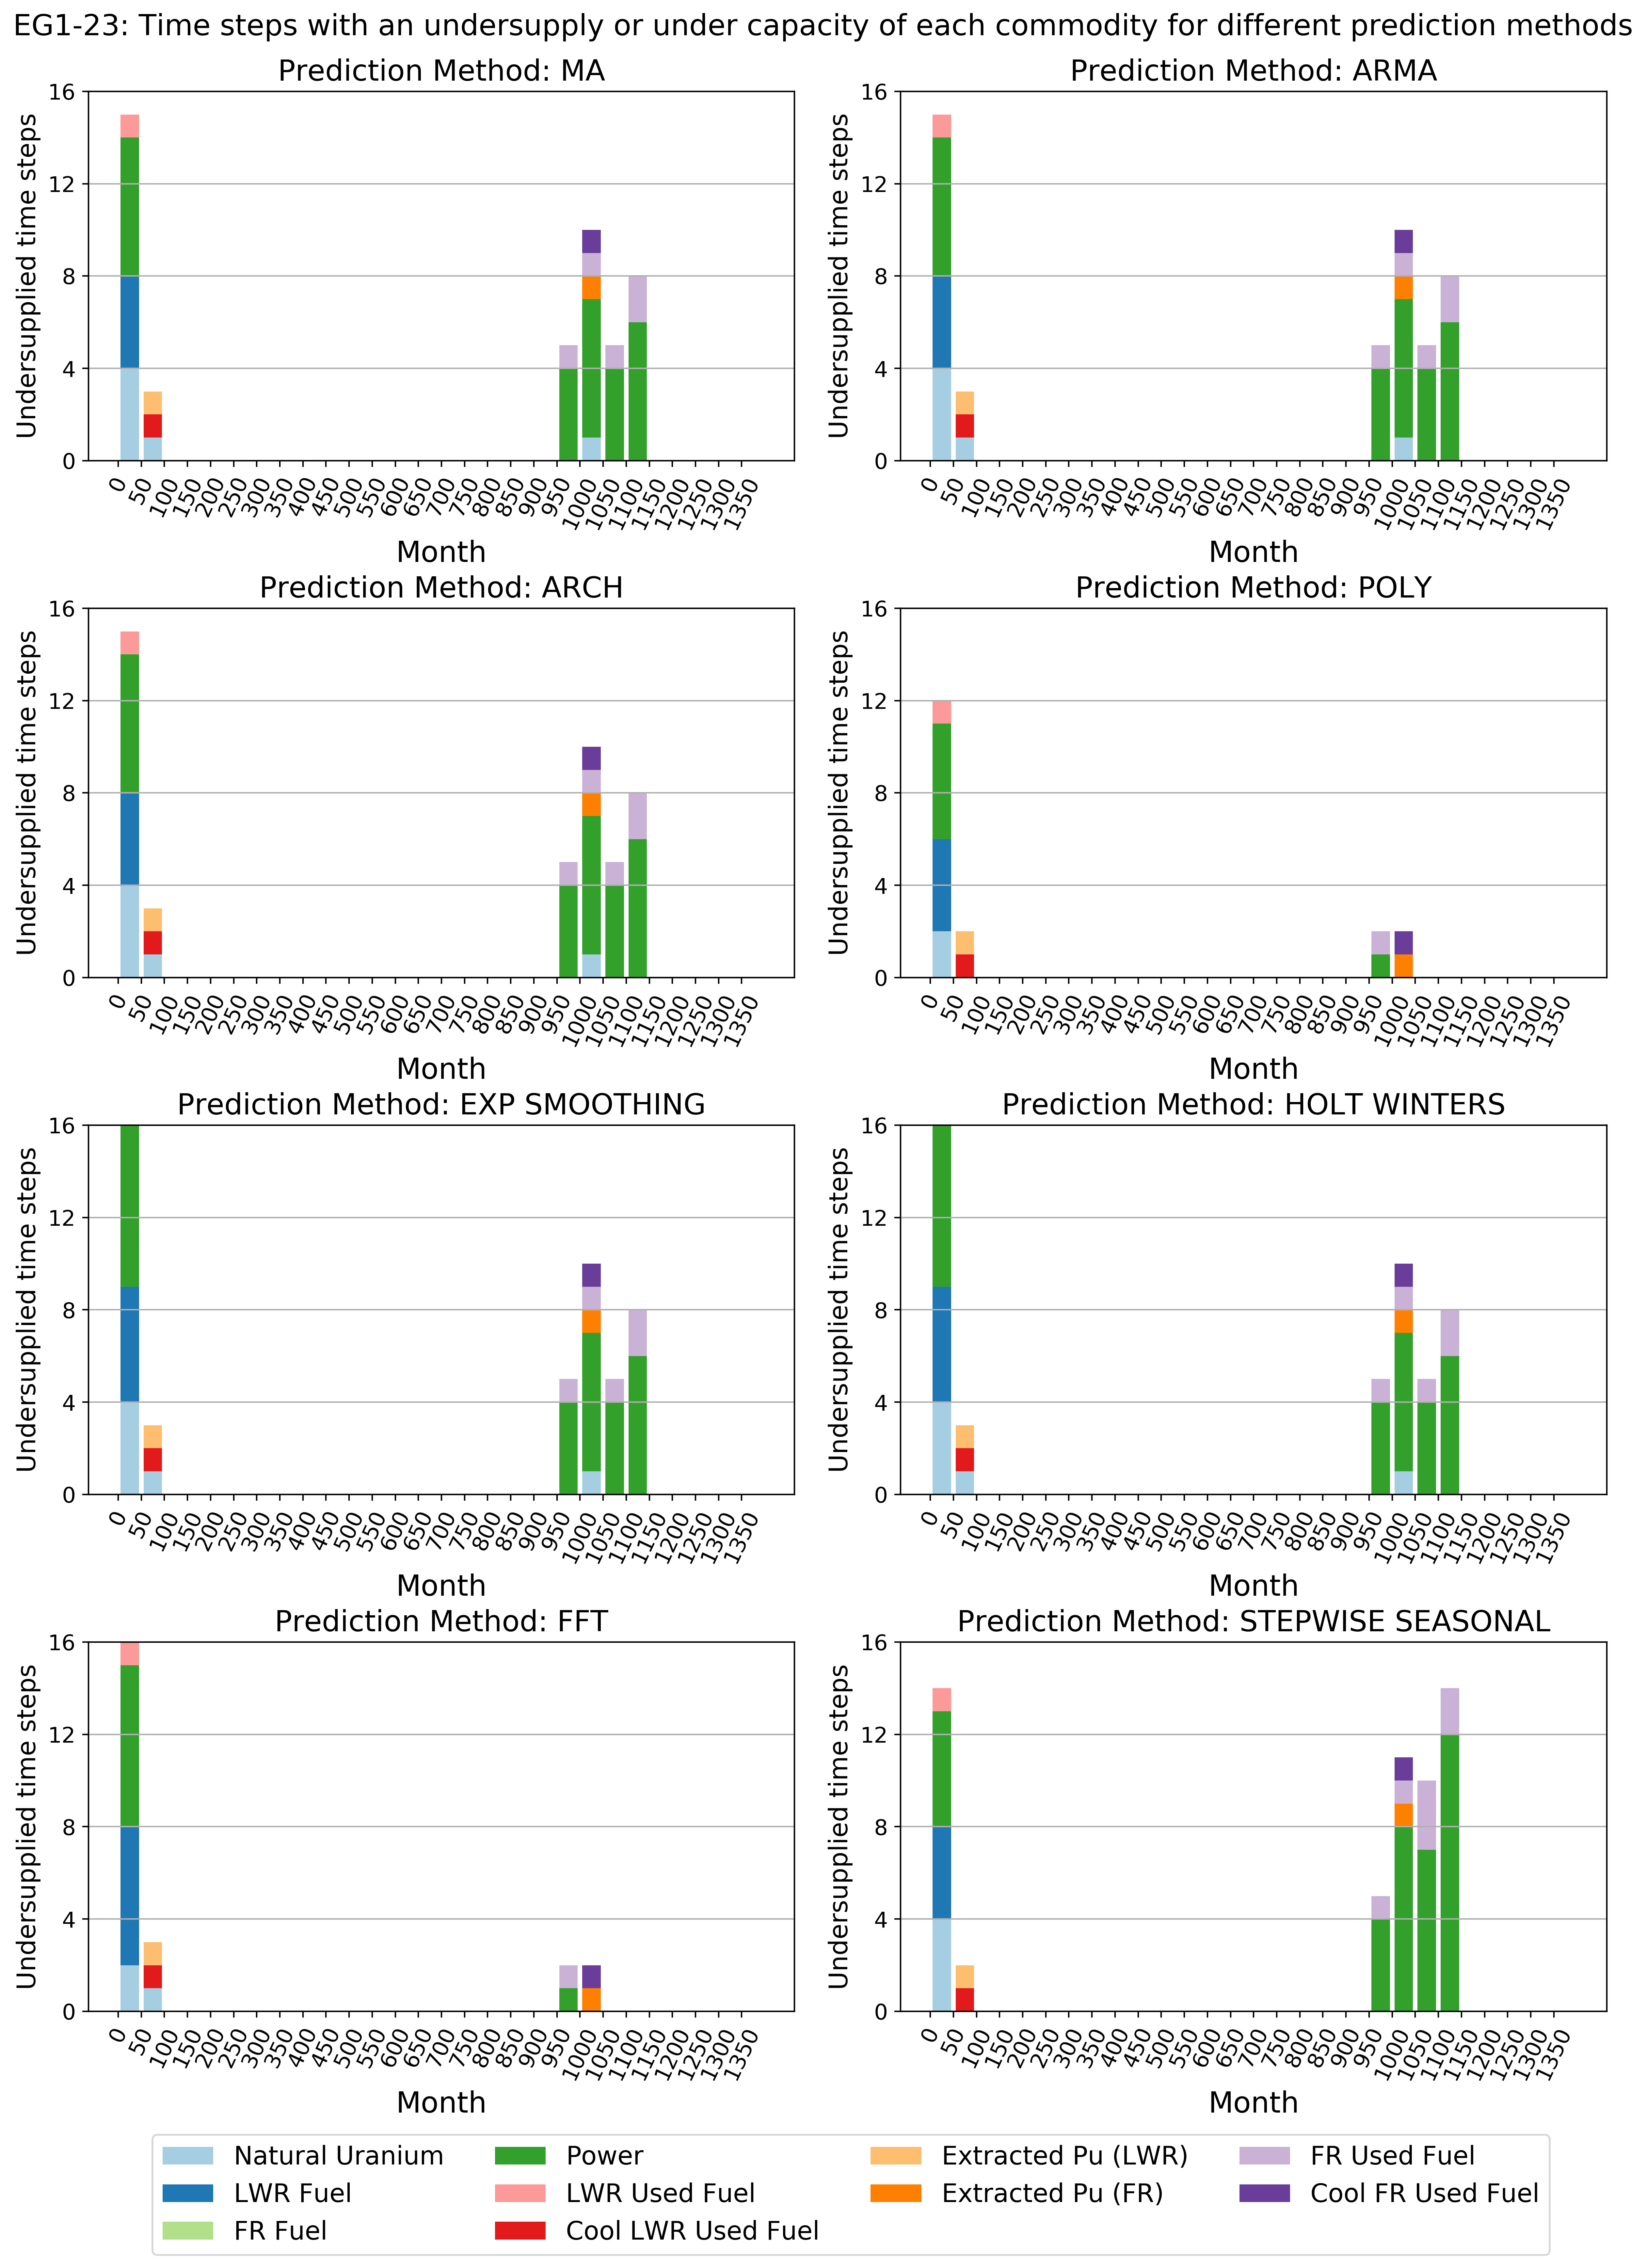
\includegraphics[width=\linewidth]{eg01-23-histogram.png} 
	\caption{
	EG01-EG23 transition scenario with constant power demand. 
	Each subplot shows the total number of time steps in which there exists 
	undersupply and under capacity of commodities for each prediction method. 
	The different colors represent different commodities and each vertical bar refers 
	to 50 time steps in the simulation.}
	\label{fig:eg23under}
\end{figure}

\begin{figure}[]
	\centering
	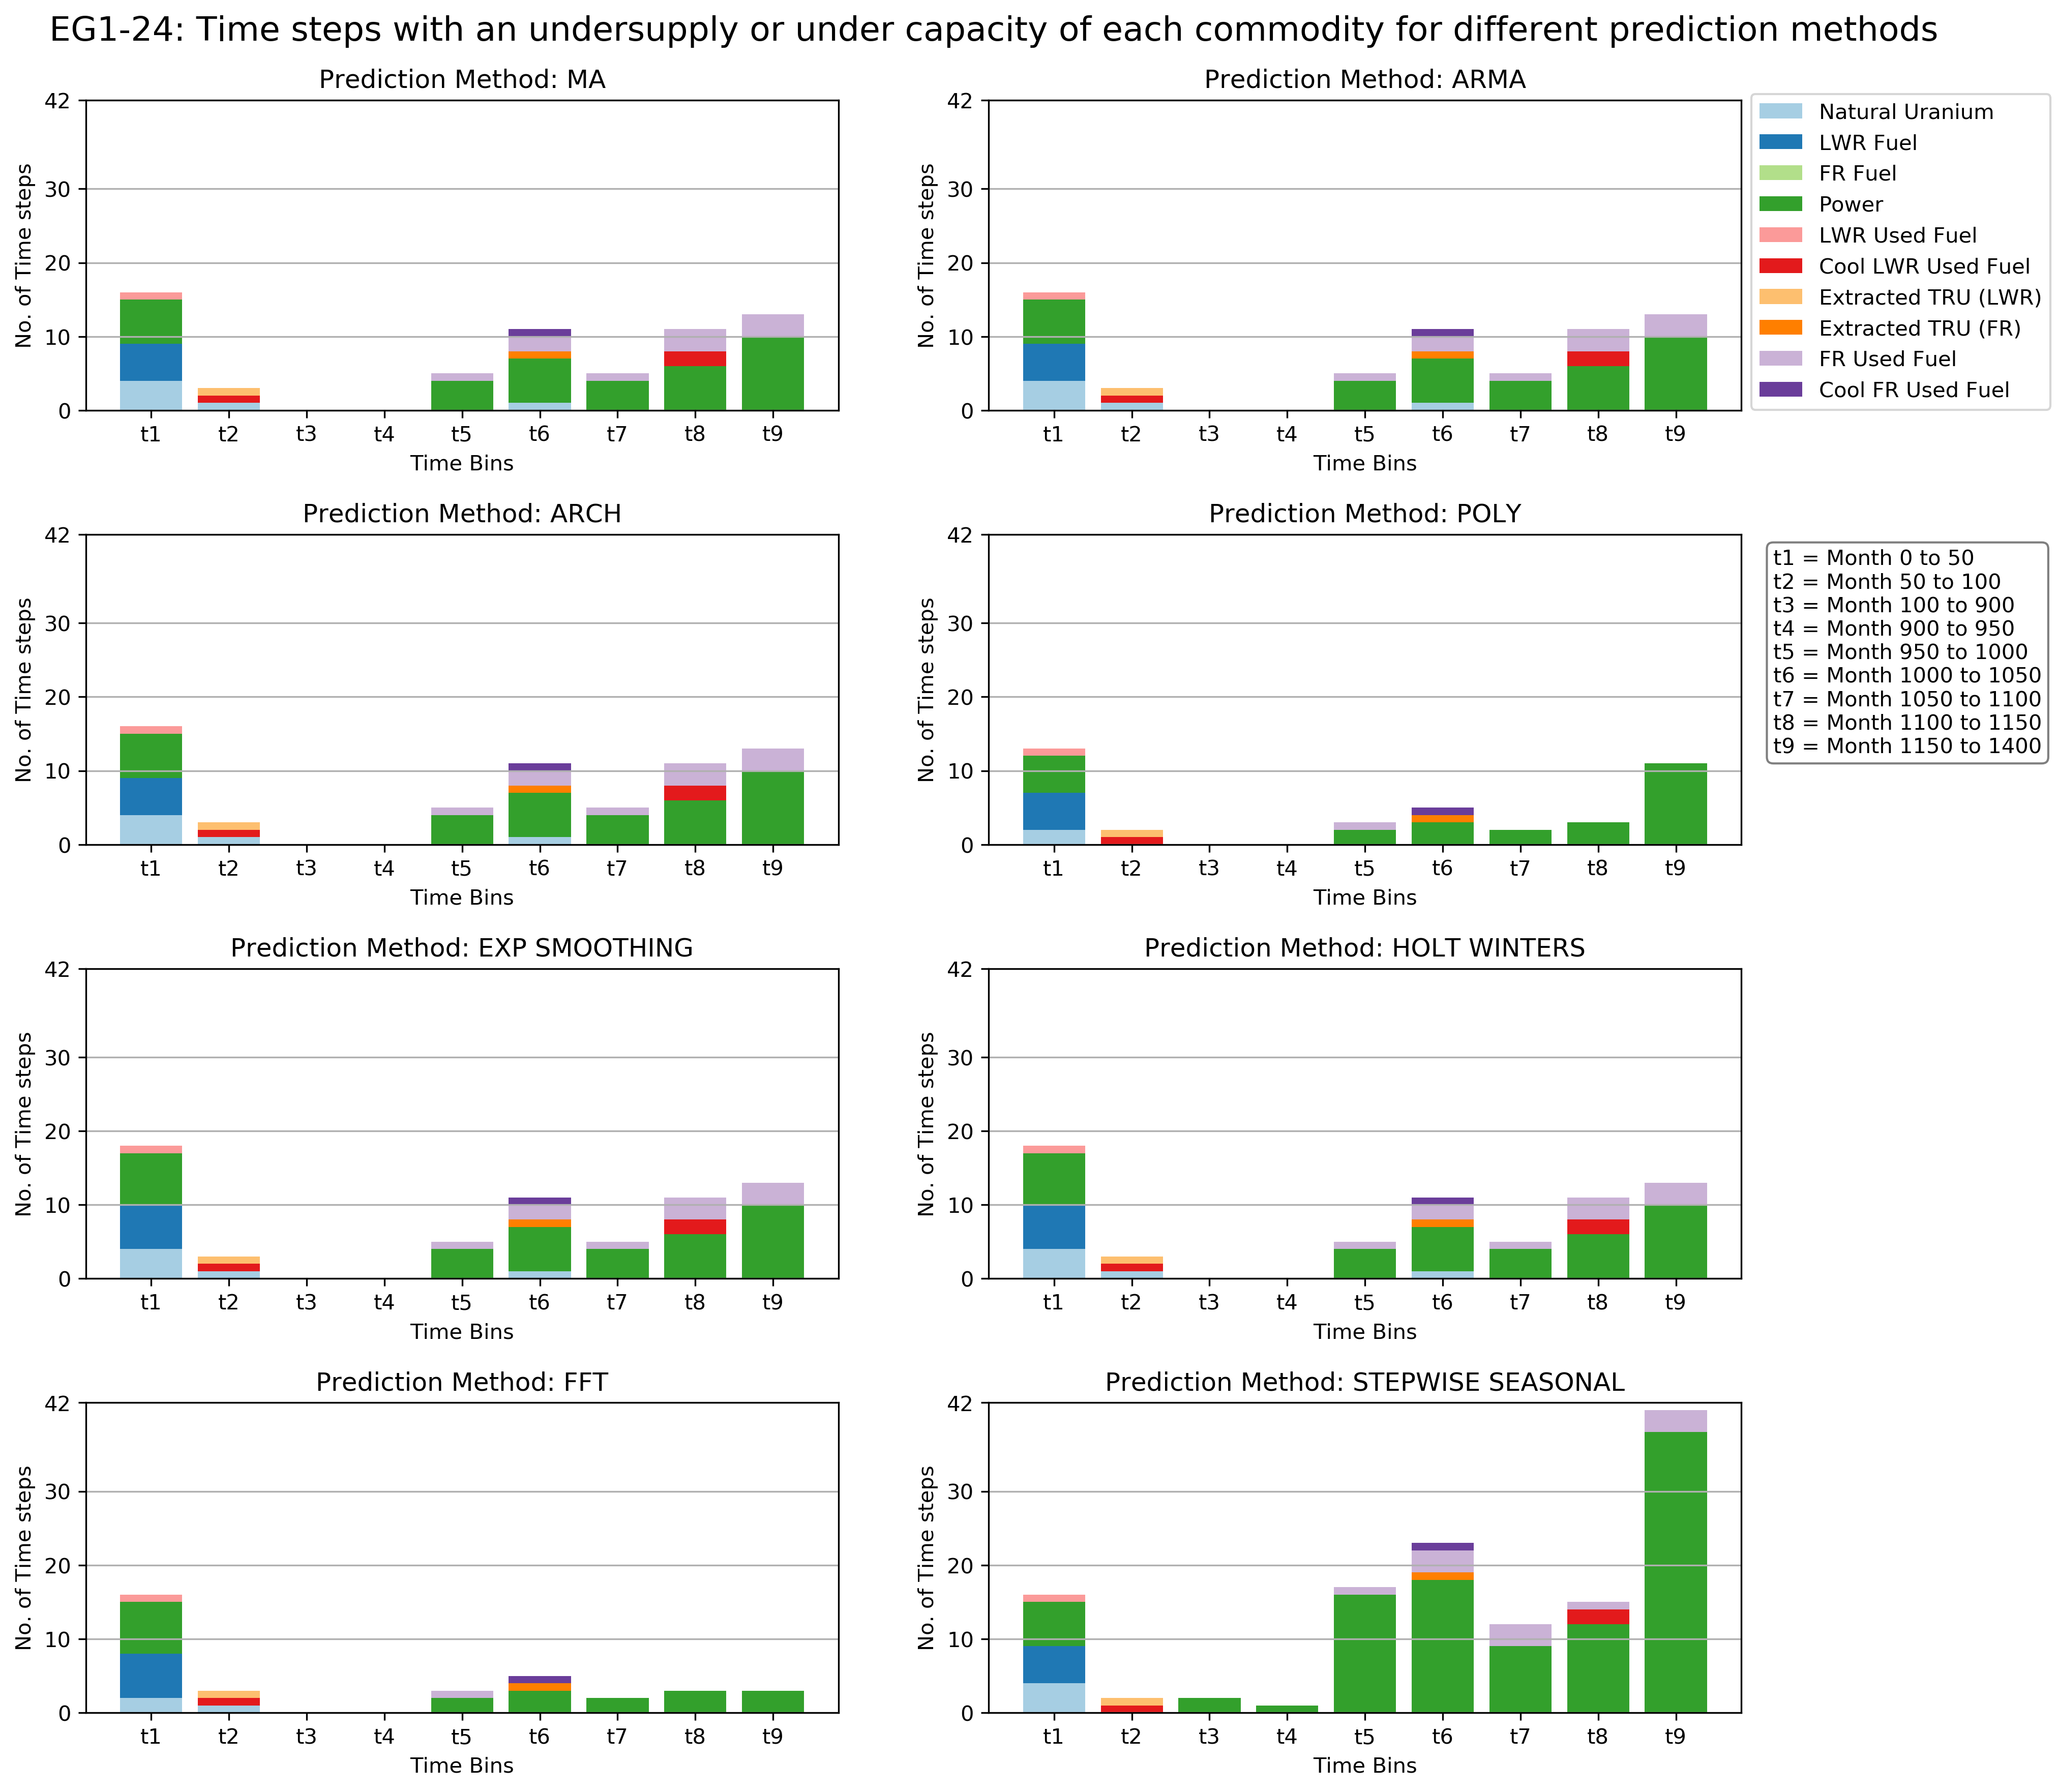
\includegraphics[width=\linewidth]{eg01-24-histogram.png} 
	\caption{
	EG01-EG24 transition scenario with linearly increasing power demand. 
	Each subplot shows the total number of time steps in which there exists 
	undersupply and under capacity of commodities for each prediction method. 
	The different colors represent different commodities and each vertical bar refers 
	to 50 time steps in the simulation.}
	\label{fig:eg24under}
\end{figure}

\begin{table}[]
	\centering
		\caption{Total number of time steps with undersupply of power for the EG01-EG23,
		EG01-EG24, EG01-EG29, and EG01-EG30 transition scenarios for different prediction methods.}
		\label{tab:all-power}
		\footnotesize
        \begin{tabularx}{\textwidth}{l|RRRR}
		\hline
		\multicolumn{5}{c}{\textbf{No. of Time Steps with Power Undersupply for Each Transition Scenario}} \\ \hline
		\textbf{Algorithm} & \textbf{EG01-EG23}  & 
		\textbf{EG01-EG24}   & \textbf{EG01-EG29} & 
		\textbf{EG01-EG30} \\ \hline
		\texttt{MA}     		    & 26 	& 36  &  15  & 24 \\ 
		\texttt{ARMA}     	    & 26 	& 36  &  15  & 24\\ 
		\texttt{ARCH}     	    &  26 	& 36  &  15  & 21\\ 
		\texttt{POLY}      		&  6 	& 65  &  4 &  9\\ 
		\texttt{EXP-SMOOTHING} 	& 27 	& 37  & 16 & 25\\ 
		\texttt{HOLT-WINTERS}  	& 27 	& 37  & 16 & 25\\ 
		\texttt{FFT}       		& 8 	& 20  & 5 & 9\\ 
		\texttt{SW-SEASONAL}    & 36 	& 107 & 14 & 51\\ \hline
	\end{tabularx}
\end{table}

Figures \ref{fig:eg23under}, \ref{fig:eg24under}, and Table 
\ref{tab:all-power} show that the \texttt{POLY} method 
performs best for constant power transition scenarios, 
and the \texttt{FFT} method performs best for linearly increasing 
power transition scenarios. 
Undersupply and under-capacity of commodities occur during two main time periods: 
initial demand for the commodity and during the transition period.
To further \deploy's primary objective of minimizing the power undersupply, 
sensitivity analysis of the power supply buffer is conducted 
with the best-performing prediction method for each transition scenario.  

\subsection{Comparison of Power Buffer Sizes}
For the EG01-EG23, EG01-EG24, EG01-EG29, and EG01-EG30 transition scenarios, 
the power buffer size is varied for the best-performing prediction method, 
which is the \texttt{POLY} method for EG01-EG23 and EG01-EG29, and the 
\texttt{FFT} method for EG01-EG24 and EG01-EG30. 
Varying the power buffer size does not impact the number of 
undersupplied time steps for the EG01-EG23 and EG01-EG29 constant 
power demand transition scenarios.
In Table \ref{tab:all-power-fin}, there are 6 and 4 time steps
in which there is power undersupply for the EG01-EG23 and EG01-EG29 
transition scenarios, respectively. 
As seen in figure \ref{fig:eg23under}, these undersupply time 
steps occur at the beginning of the simulation and for one 
time step when the transition begins. 
We expected this since without time-series data 
at the beginning of the simulation, \deploy takes a few 
time steps to collect time-series data about power demand 
to predict and start deploying reactors and supporting 
fuel cycle facilities. 
When the transition begins, power is undersupplied for one 
time step, following this, \deploy accounts for the 
undersupply by deploying facilities to meet power demand.
Therefore, we minimized the power undersupply for constant 
power EG01-EG23 and EG01-EG29 transition scenarios with 
a 0MW power supply buffer. 

We varied the power buffer size for the EG01-EG24 and EG01-EG30 
linearly increasing power demand transition scenarios. 
Figures \ref{fig:eg24-bufplot}, \ref{fig:eg30-bufplot}, 
and Table \ref{tab:buff_size} 
show that increasing the buffer size increases the robustness 
of the supply chain by minimizing power undersupply. 
The cumulative undersupply is minimized with a 6000MW and 8000MW 
buffer for EG01-EG24 and EG01-EG30 respectively.
In Figure \ref{fig:eg24-bufplot}, a 4000MW buffer size has 
8 time steps with undersupply, while a 6000MW buffer size has 
7 time steps with undersupply. 
In Figure \ref{fig:eg30-bufplot}, a 2000MW buffer size has 
6 time steps with undersupply, while a 8000MW buffer size has 
5 time steps with undersupply. 
We determined that extra commissioning of multiple reactors does not 
justify a single time step with no undersupply. 
This type of logic is difficult to program into a NFC simulator, 
therefore, even though NFC simulators can help inform policy decisions, 
decision-makers must still evaluate NFC simulator results to determine if 
they are valid and logical. 
Therefore, a buffer of 4000MW and 2000MW minimizes 
the power undersupply for EG01-EG24 and EG01-EG30 transition 
scenarios, respectively.

\begin{table}[]
	\centering
        \caption{Undersupply/capacity of key commodities for the best performing EG01-EG23, EG24, EG29, EG30 transition scenarios.}
		\label{tab:all-power-fin}
		\footnotesize
        \begin{tabular}{lcccc}
		\hline
		& \multicolumn{3}{c}{\textbf{No. of Time Steps with Undersupply}} \\ \hline
		\textbf{Transition Scenario} & EG01-EG23 & 
		EG01-EG24 & EG01-EG29 & EG01-EG30 \\ \hline 
		\textbf{Commodities} \\ 
		Natural Uranium		    & 2 	& 3  &  1  & 1 \\ 
		\gls{LWR} Fuel     	    & 4 	& 6  &  1  & 2\\ 
		\gls{SFR} Fuel     	    &  0 	& 0  &  2  & 2\\ 
		\gls{MOX} \gls{LWR} Fuel &-&-&2&2 \\
		Power      				&  6 	& 7  &  4 &  5\\ 
		\gls{LWR} Spent Fuel	& 1 	& 1  & 1 & 1\\ 
		\gls{SFR} Spent Fuel     	    &  1 	& 1  &  1  & 1\\ 
		\gls{MOX} \gls{LWR} Spent Fuel &-&-&1&1 \\ \hline 
	\end{tabular}
\end{table}

\begin{figure}[]
	\centering
	\begin{subfigure}[t]{\textwidth}
		\centering
		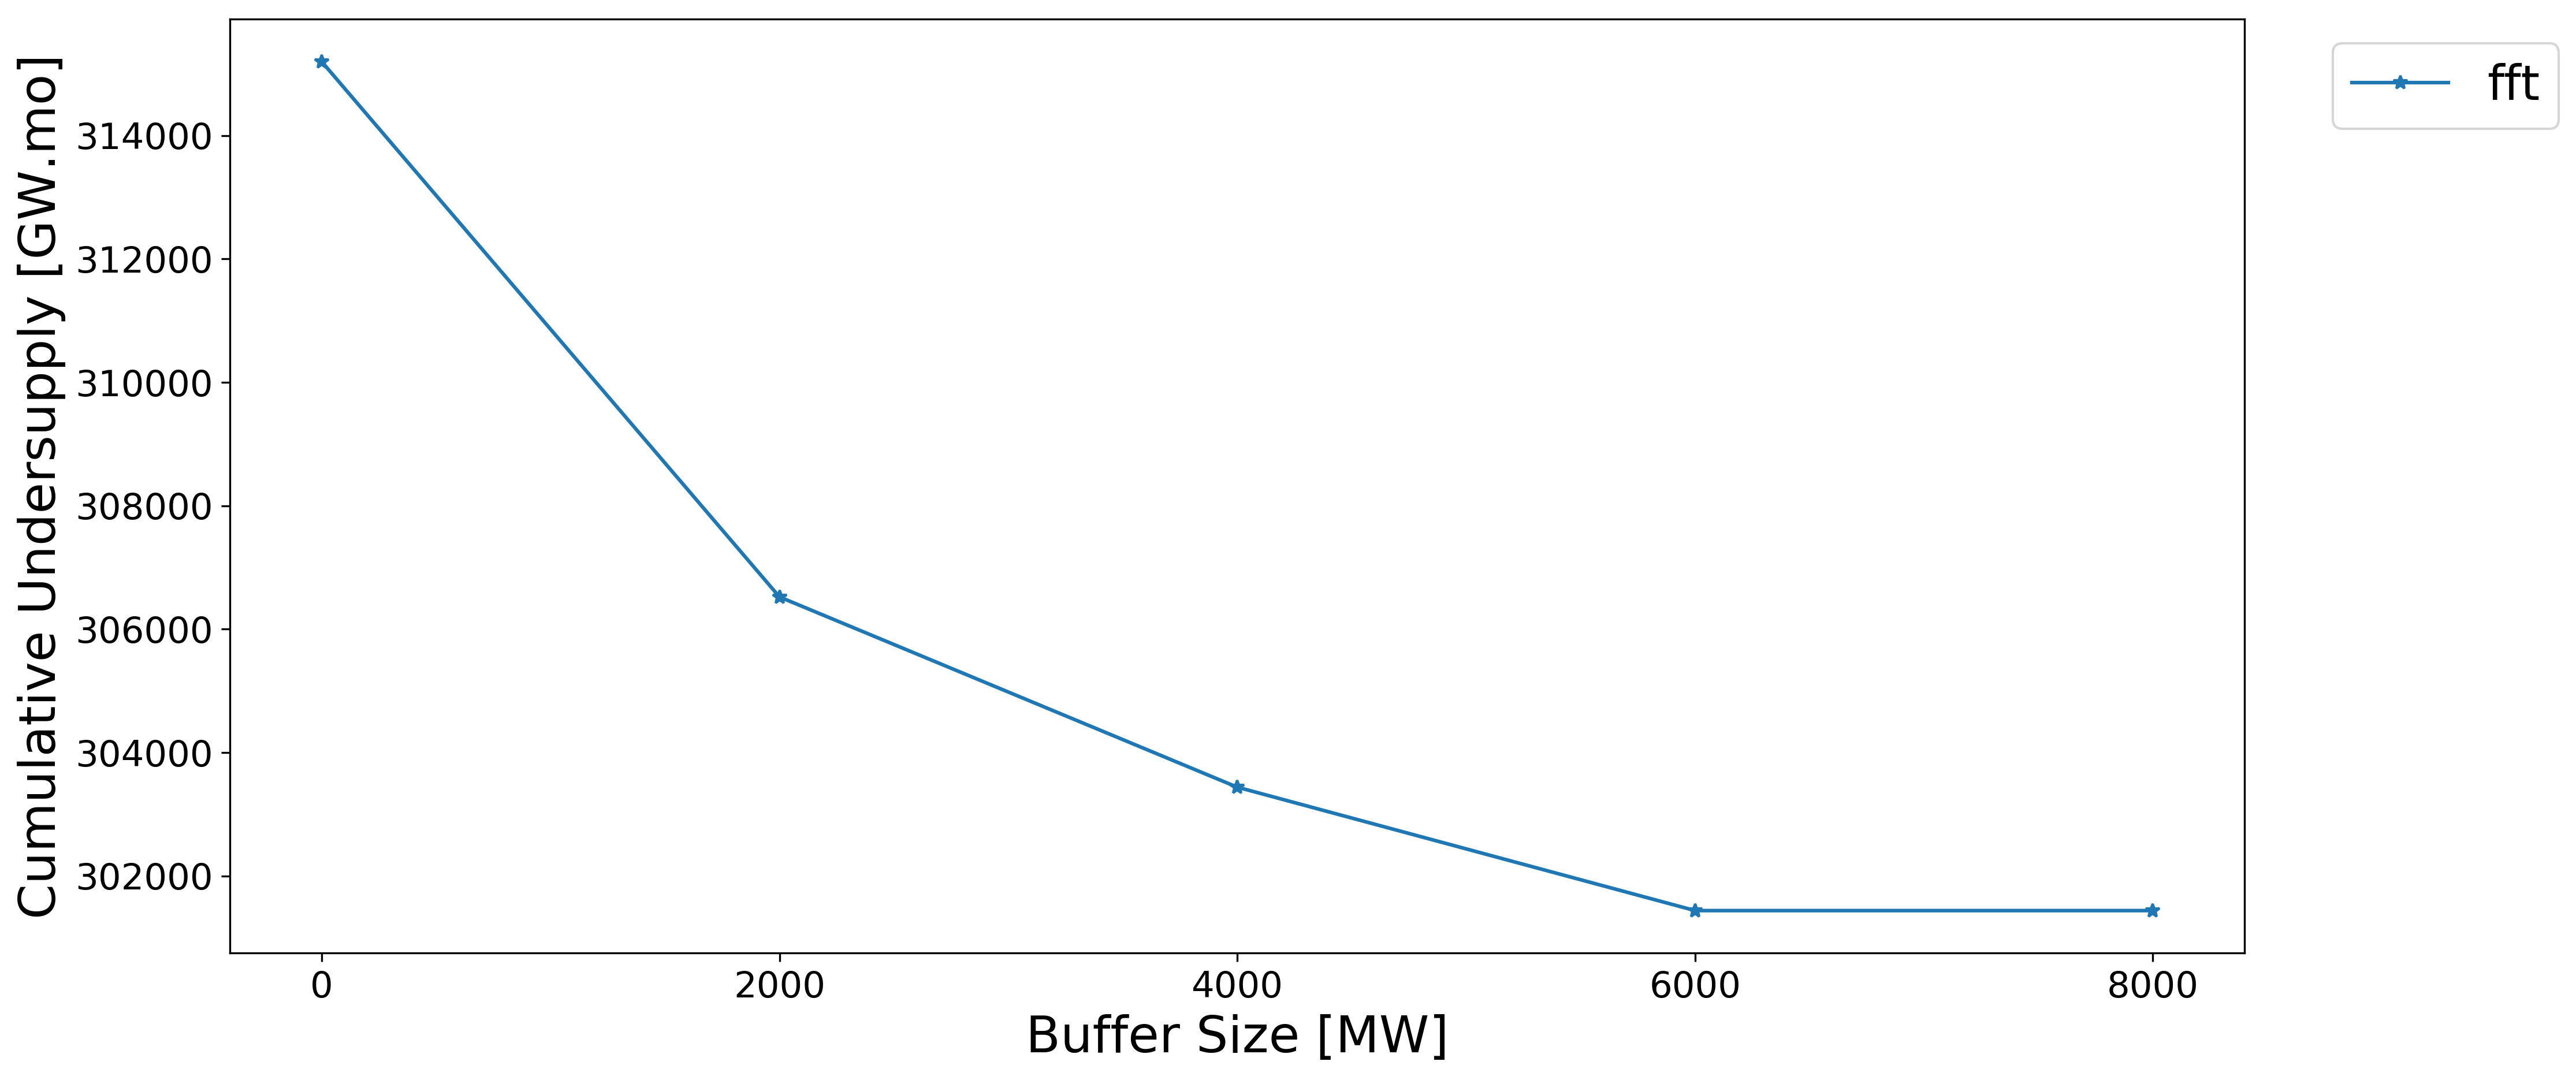
\includegraphics[width=0.75\linewidth]{24-sens-buffer.png} 
		\caption{EG01-EG24: Power buffer size vs. cumulative undersupply}
		\label{fig:eg24-bufplot}
	\end{subfigure}
	\begin{subfigure}[t]{\textwidth}
		\centering
		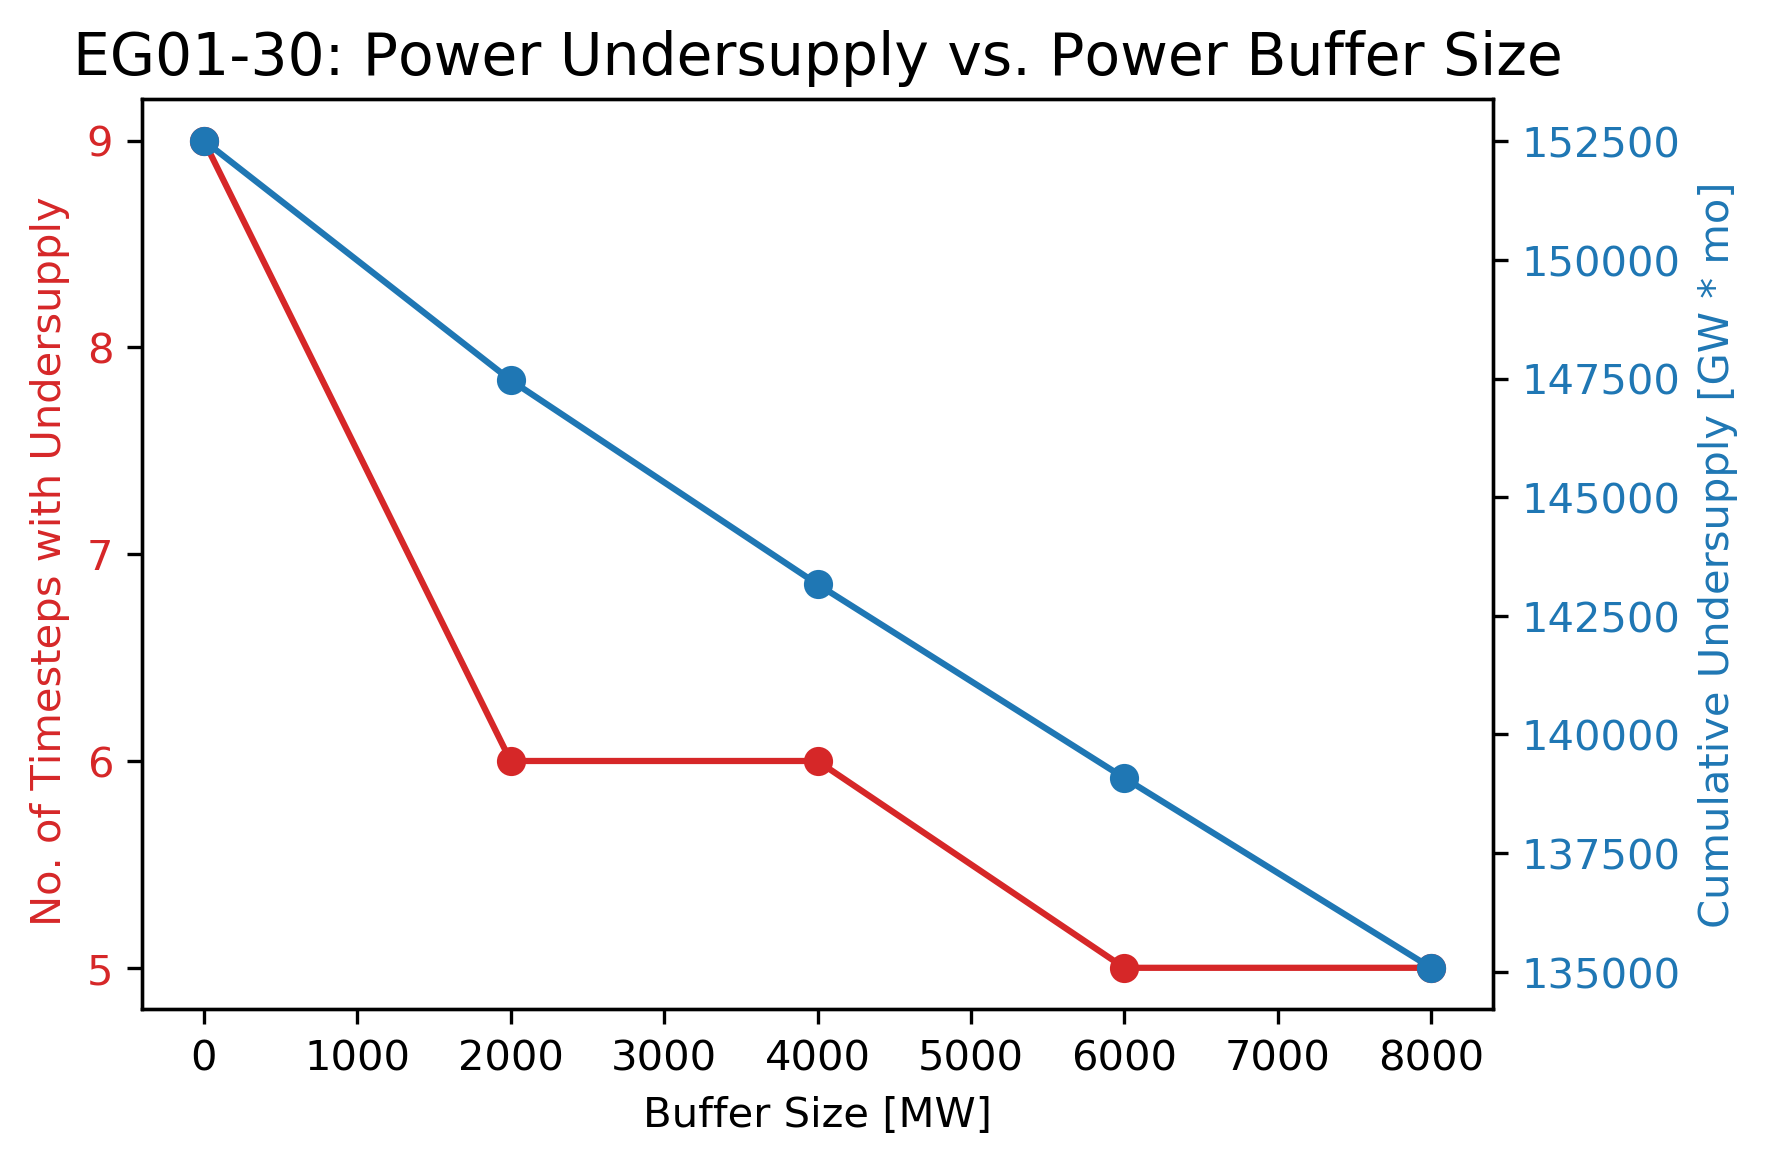
\includegraphics[width=0.75\linewidth]{30-sens-buffer.png} 
		\caption{EG01-EG30: Power buffer size vs. cumulative undersupply}
		\label{fig:eg30-bufplot}
	\end{subfigure}
	\hfill
	\caption{The effect of sensitivity analysis of power buffer size on cumulative 
	undersupply of power for EG01-EG24 and EG01-EG30 transition scenarios 
	with linearly increasing power demand using the \texttt{FFT} prediction method.}
	\label{fig:sabuffer}
\end{figure}

\begin{table}[]
	\centering
	\caption{The effect of sensitivity analysis of power buffer size on cumulative 
	undersupply of power for EG01-EG24 and EG01-EG30 transition scenarios with linearly 
	increasing power demand using the \texttt{FFT} prediction method.}
	\label{tab:buff_size}
	\footnotesize
		\begin{tabular}{r|lrr}
                \hline
        \textbf{Buffer [MW]}     & \textbf{Undersupply}             & \textbf{EG01-EG24}   & \textbf{EG01-EG30} \\
		\hline
		\textbf{0}             & Time steps $[\#]$ & 20 & 9\\  
                      & Energy $[GW\cdot mo]$    & 315791 & 152517 \\ \hline
		\textbf{2000}          & Undersupplied $[\#]$ & 9 & 6 \\  
        	      & Energy $[GW\cdot mo]$    & 306520 & 147166 \\ \hline
        \textbf{4000}          & Time steps $[\#]$ & 8 & 6 \\  
				  & Energy $[GW\cdot mo]$    & 303438 & 143166 \\ \hline
		\textbf{6000}          & Time steps $[\#]$ & 7 & 5 \\  
		& Cumulative $[GW]$    & 303438 & 139083 \\ \hline
        \textbf{8000}          & Time steps $[\#]$ & 7 & 5  \\  
	              & Energy $[GW\cdot mo]$    & 303438 & 135083 \\ \hline
	\end{tabular}
\end{table}

\subsection{Best Performance Models}
Table \ref{tab:bestinputs} shows the \deploy input parameters for
EG01-EG23, EG01-EG24, EG01-EG29, and EG01-EG30 transition scenarios
that minimize the undersupply of power as well as the
undersupply and under-capacity of the other commodities
in the simulation. 
The need for commodity supply buffers is a reflection of reality
in which a supply buffer is usually maintained to ensure 
continuity in the event of an unexpected failure in the supply chain
\cite{united_nations_institute_for_disarmament_research_multilateralization_2013}.

Figures \ref{fig:23stack} and \ref{fig:30stack} show
time-dependent deployment of reactor and supporting facilities for 
the EG01-EG23 constant power demand and EG01-EG30 linearly increasing power demand 
transition scenarios, respectively. 
\deploy automatically deploys reactor and supporting facilities 
to set up a supply chain to meet power demand
during a transition from \glspl{LWR} to \glspl{SFR} for EG01-EG23, 
and from \glspl{LWR} to \gls{MOX} \glspl{LWR} and \glspl{SFR} for 
EG01-EG30. 
EG01-EG24 and EG01-EG29 facility deployment plots are similar to 
EG01-EG23 and EG01-EG30, respectively, therefore they are not shown. 

\begin{table}[]
	\centering
	\resizebox{\textwidth}{!}{
	\begin{tabular}{r|cccc}
	\hline
	\multicolumn{1}{c|}{\multirow{2}{*}{\textbf{Input Parameter}}} & \multicolumn{4}{c}{\textbf{Simulation Description}}                                                                                                                                                                                                                                                       \\ \cline{2-5}
	\multicolumn{1}{c|}{}                                          & \multicolumn{1}{l}{\textbf{EG01-EG23}}                                                                 & \textbf{EG01-EG24}                  & \textbf{EG01-EG29}                 &\textbf{EG01-EG30}                                                  \\ \hline
	\textbf{Demand Driving}                                      & Power & Power & Power & Power                                                                                                                                                                                                                                                                                \\ 
	\textbf{Commodity} \\ \hline  
	\textbf{Demand}                                               & 60000                                                                                & 60000 & 60000                     &  60000                                        \\ 
	\textbf{Equation [MW]} & &$+250t/12$& &$+250t/12$ \\ \hline 
	\textbf{Prediction}                                             & \texttt{POLY}       & \texttt{FFT}             & \texttt{POLY}         &  \texttt{FFT}    \\ 
	\textbf{Method} \\ \hline 
	\textbf{Deployment}   & Installed & Installed  & Installed   & Installed    \\                                                                                                                                                                                 
	\textbf{Driving Method} & Capacity & Capacity  & Capacity   & Capacity \\ \hline 
	\textbf{Fleet Share} &  MOX: 85\% &  MOX: 85\% &  MOX: 85\% &  MOX :85\%     \\
	\textbf{Percentage} &SFR: 15\%&SFR: 15\%&SFR: 15\%&SFR: 15\%\\ \hline
	\textbf{Buffer type}                                                    & \multicolumn{4}{c}{Absolute}                                                                                                                                                                                                                                                               \\ \hline
	\textbf{Power Buffer}                                                  & 0 & 4000 & 0 & 2000 \\ 
	\textbf{Size [MW]} \\ \hline \end{tabular}}
	\caption{\deploy's input parameters for EG01-EG23, EG01-EG24, EG01-EG29, and 
	EG01-EG30 transition scenarios
	that minimizes undersupply of power and minimizes 
	the undersupply and under-capacity of the other facilities. }
	\label{tab:bestinputs}
	\end{table}

\begin{figure}[]
	\centering
	\begin{subfigure}[t]{1\textwidth}
		\centering
		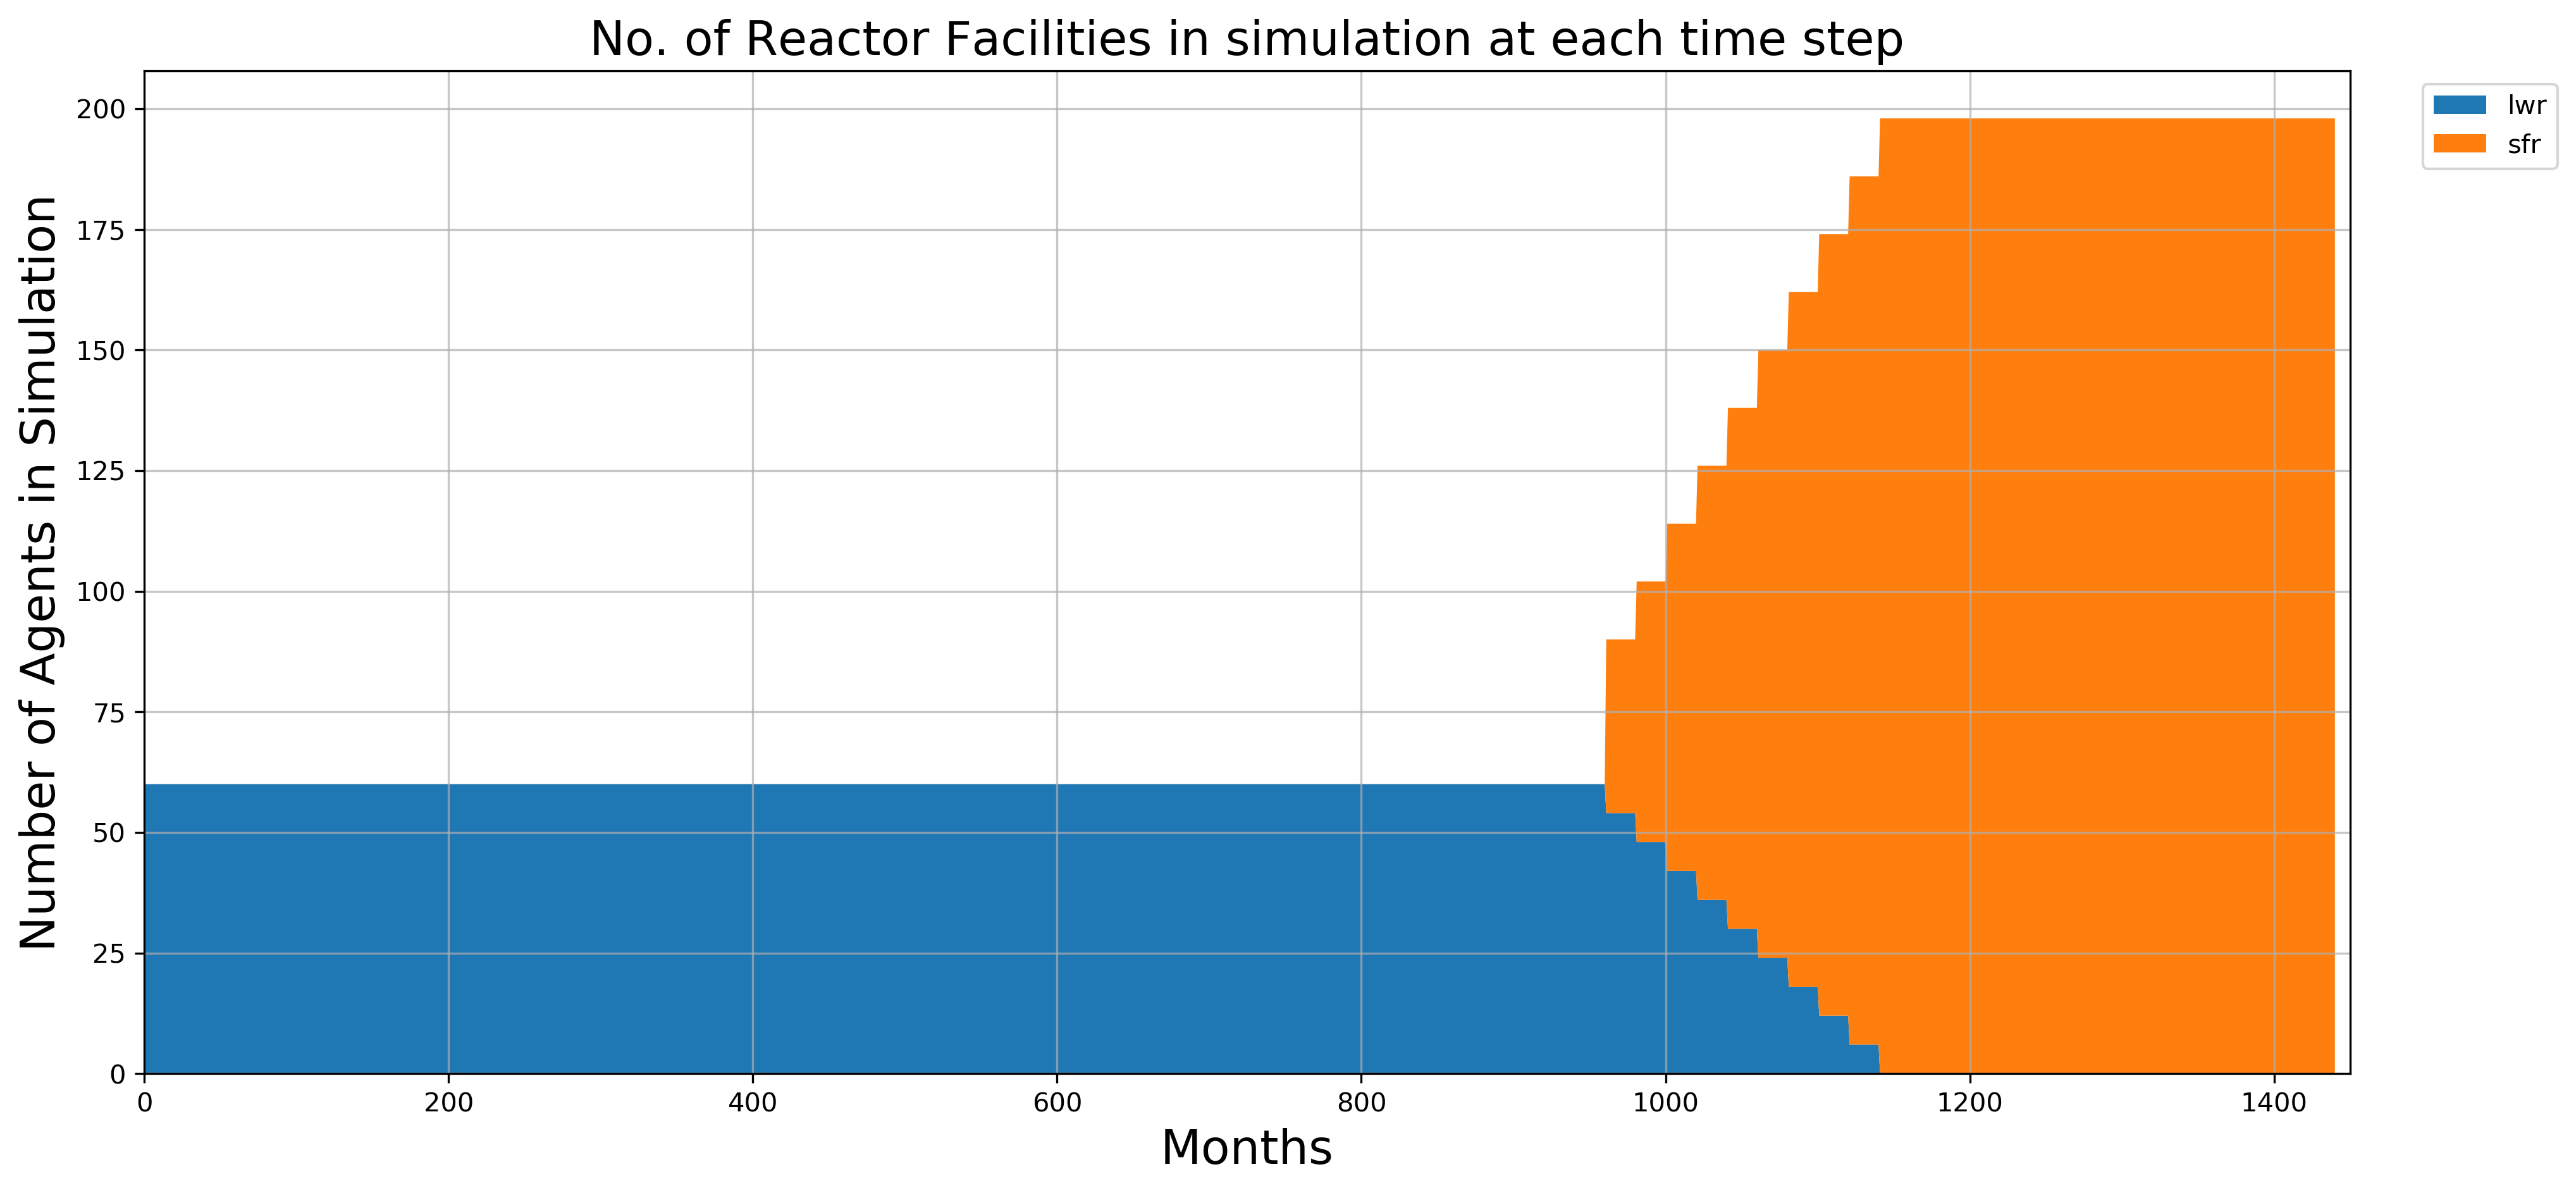
\includegraphics[width=\linewidth]{eg23-stack_reactor.png} 
		\caption{EG01-EG23: Reactor Deployment}
		\label{fig:23reactor}
	\end{subfigure}
	\begin{subfigure}[t]{1\textwidth}
		\centering
		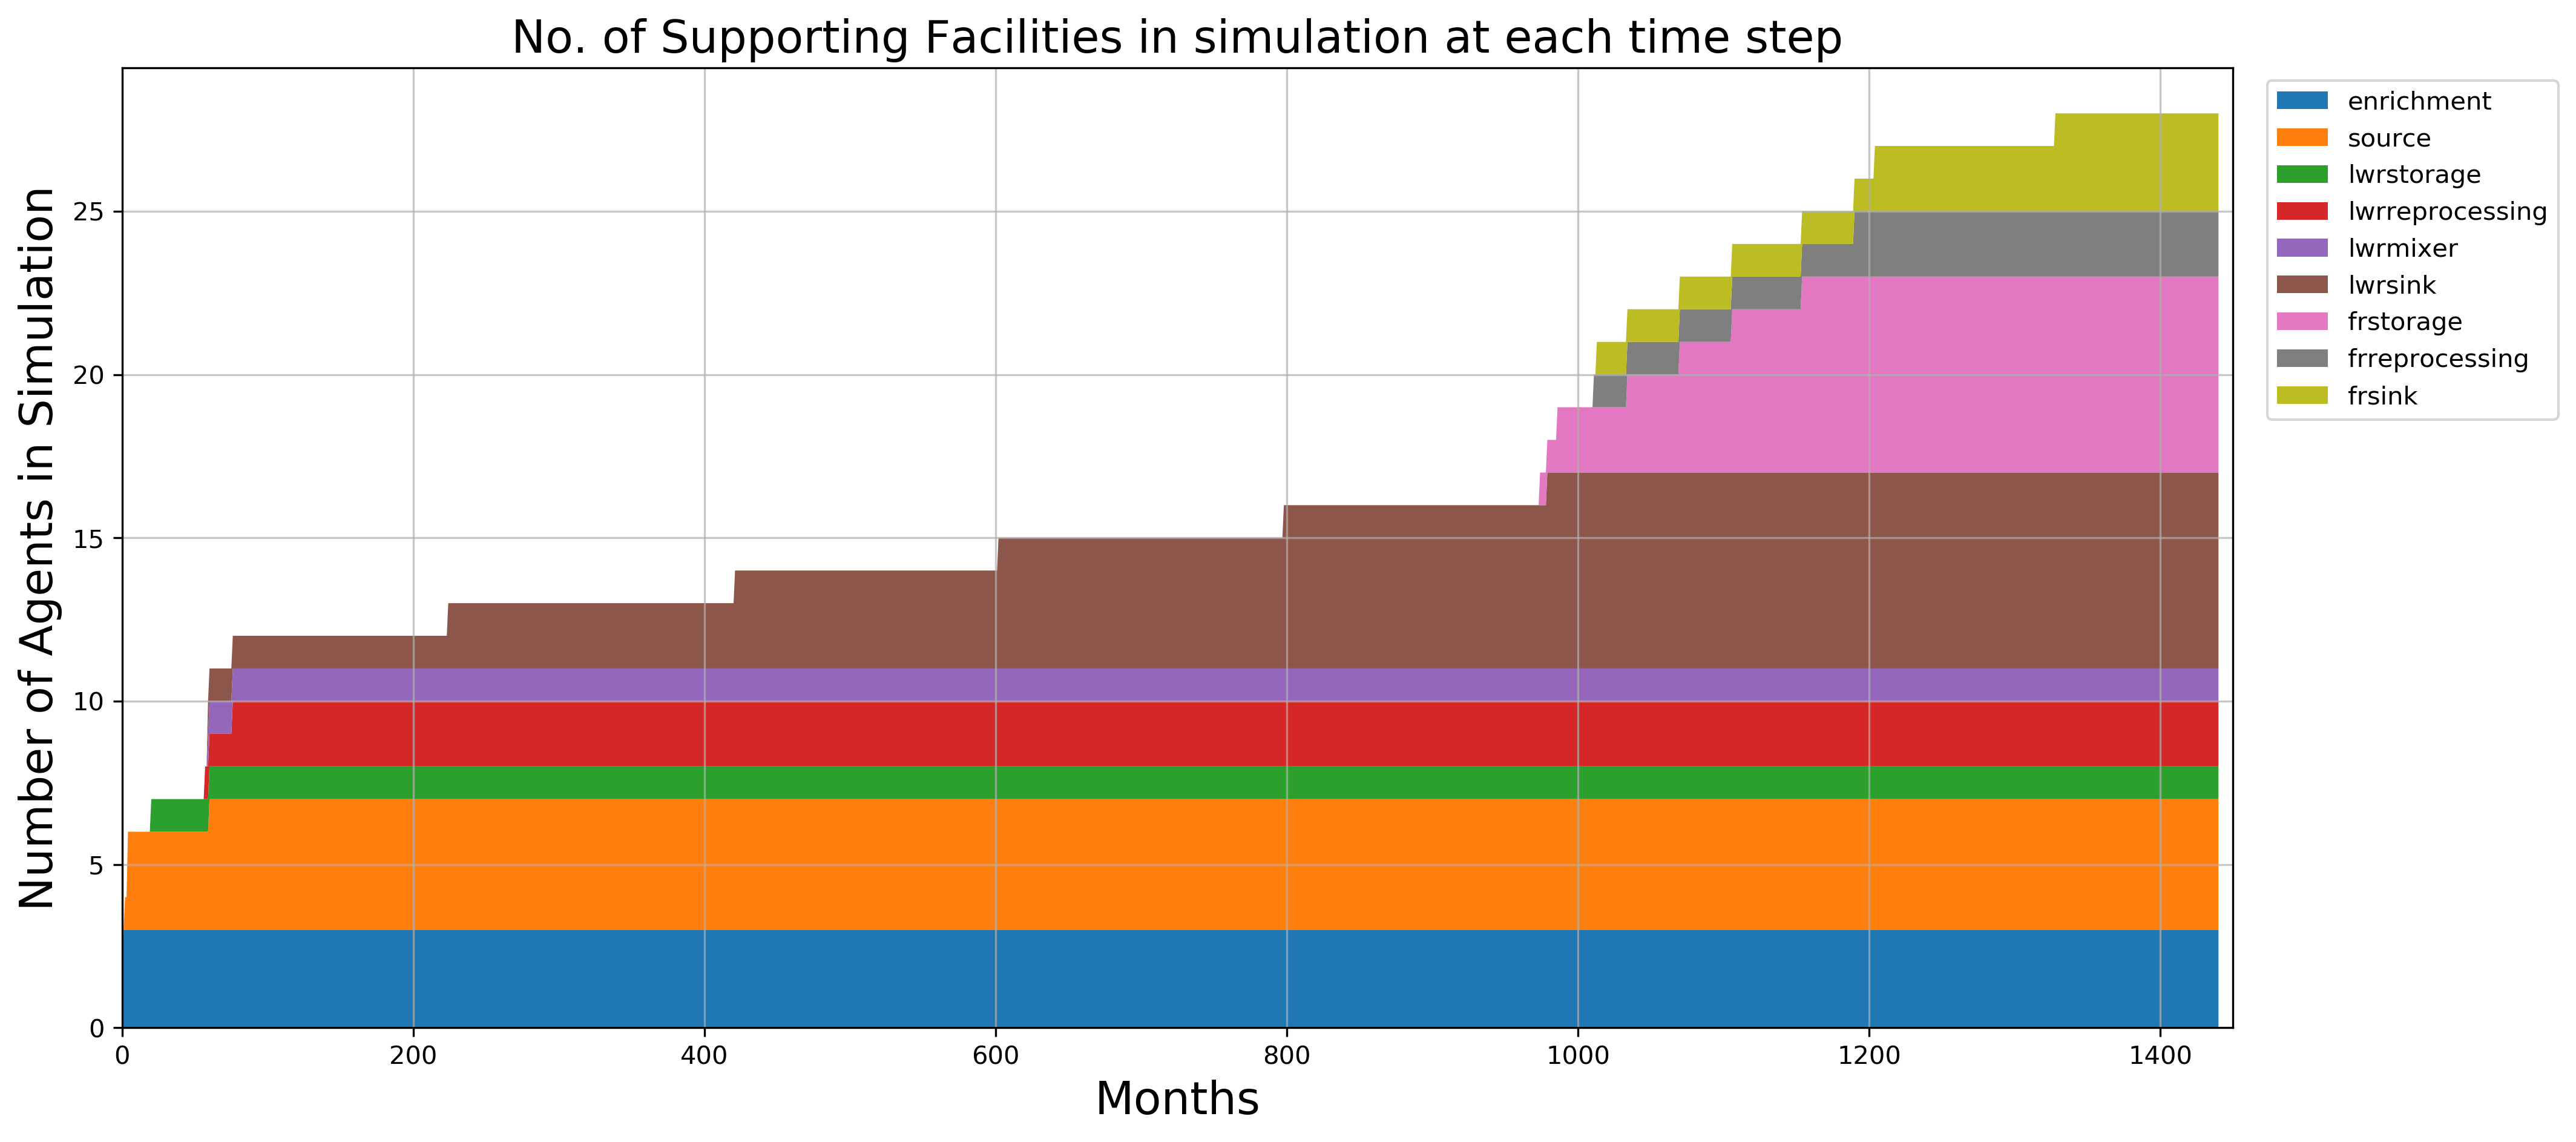
\includegraphics[width=\linewidth]{eg23-stack_support.png} 
		\caption{EG01-EG23: Supporting Facility Deployment}
		\label{fig:23support}
	\end{subfigure}
	\hfill
	\caption{Time dependent deployment of reactor and supporting facilities in 
	the EG01-EG23 constant power demand transition scenario. 
	\deploy automatically deploys reactor and supporting facilities 
	to setup a supply chain to meet constant power demand of $60000$ MW
	during a transition from \glspl{LWR} to \glspl{SFR}. }
	\label{fig:23stack}
\end{figure}

\begin{figure}[]
	\centering
	\begin{subfigure}[t]{1\textwidth}
		\centering
		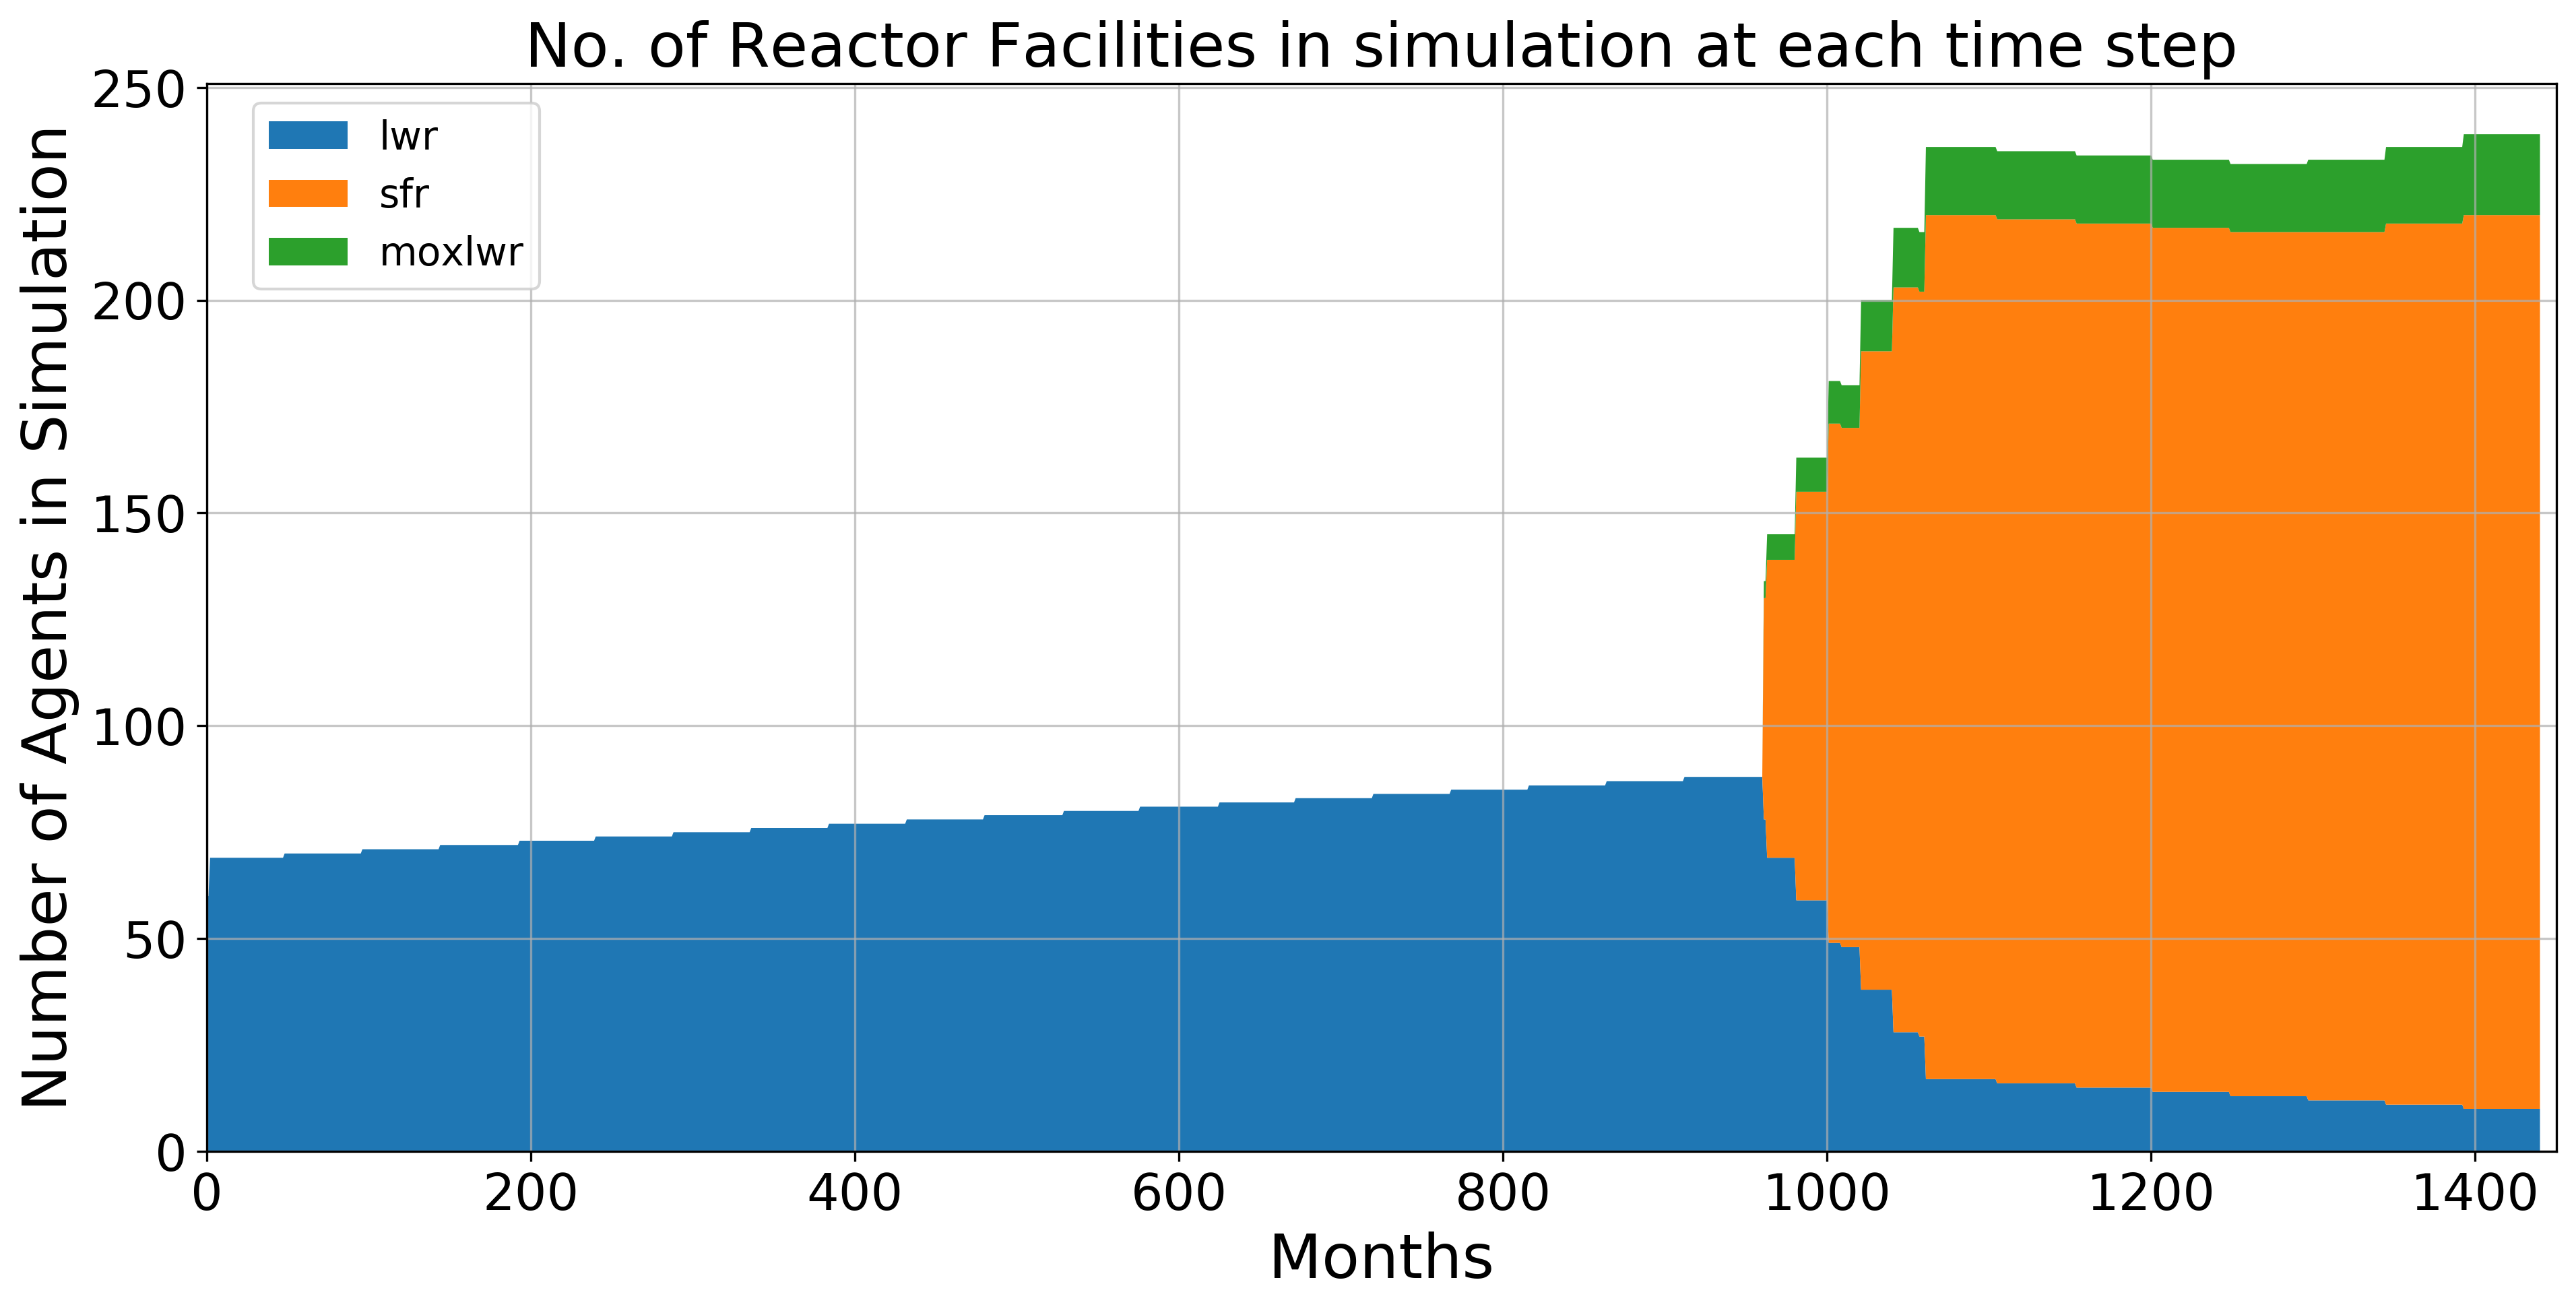
\includegraphics[width=\linewidth]{eg30-stack_reactor.png} 
		\caption{EG01-EG30: Reactor Deployment}
		\label{fig:30reactor}
	\end{subfigure}
	\begin{subfigure}[t]{1\textwidth}
		\centering
		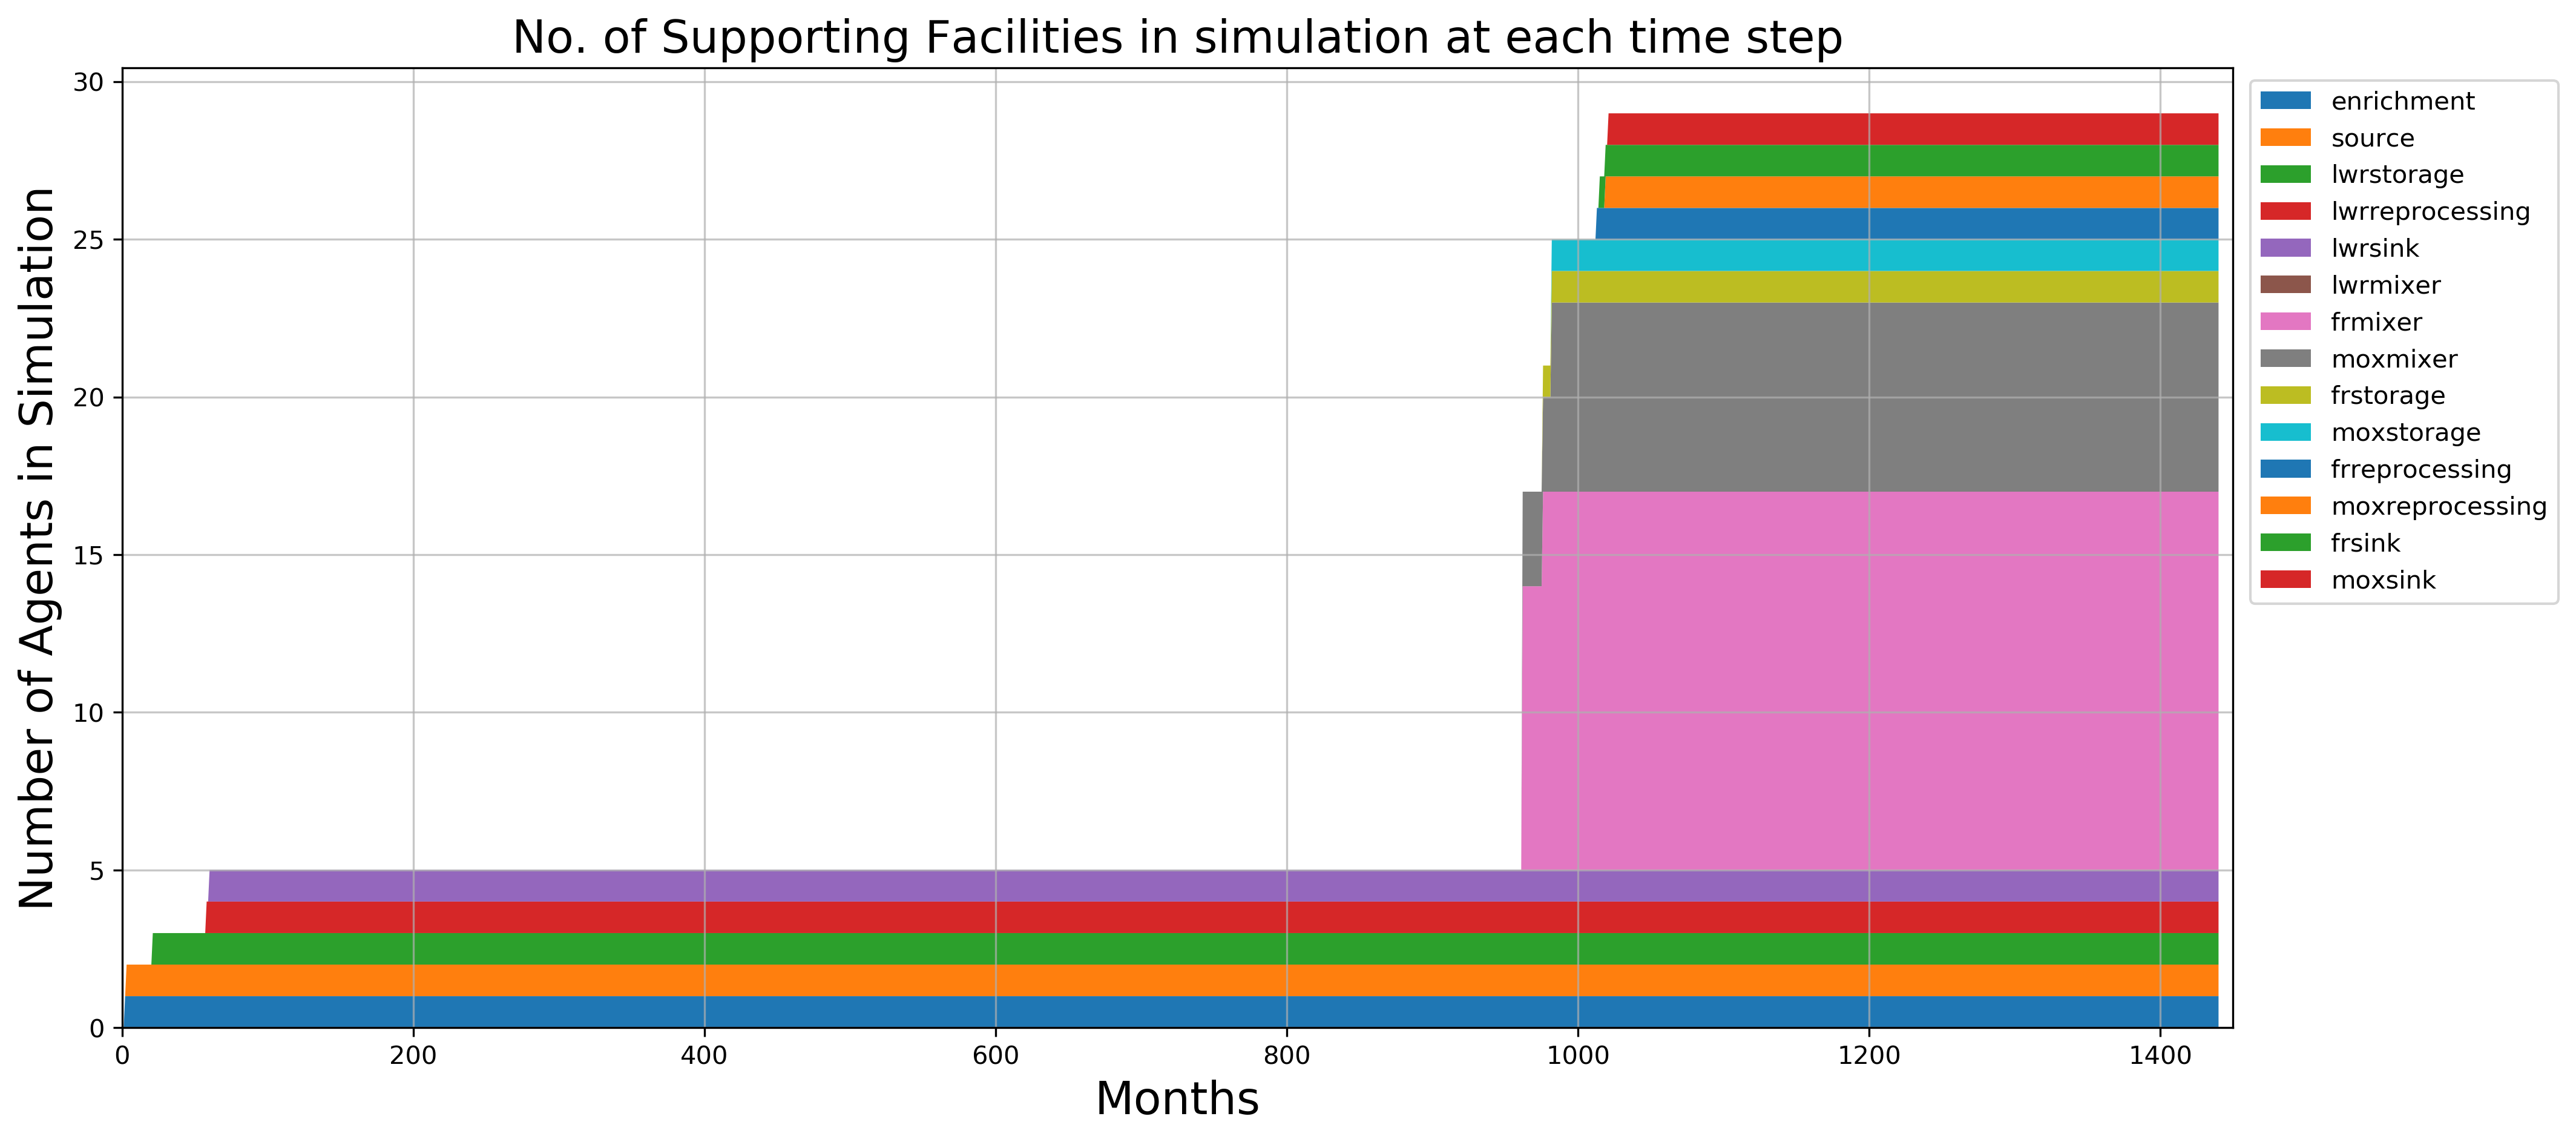
\includegraphics[width=\linewidth]{eg30-stack_support.png} 
		\caption{EG01-EG30: Supporting Facility Deployment}
		\label{fig:30support}
	\end{subfigure}
	\hfill
	\caption{Time dependent deployment of reactor and supporting facilities in 
	the EG01-EG30 linearly increasing power demand transition scenario. 
	\deploy automatically deploys reactor and supporting facilities 
	to setup a supply chain to meet linearly increasing power demand of $60000 + 250t/12$ MW
	during a transition from \glspl{LWR} to MOX LWRs and \glspl{SFR}. }
	\label{fig:30stack}
\end{figure}
